%本章研究backorder对改进效果的影响

\chapter{Backorder对改进效果的影响}

作为供应商,如果不能按时交货,有时需要将订单记下,尽快补货,并且承受一定的惩罚。这种订单称为backorder。本章中,我们将讨论backorder对我们的方案改进效果的影响。




\section{考虑Backorder成本的任意更新过程}

以汽车保险杠的生产线为例,为了使讨论简化,我们假设注塑环节需要的时间远大于喷涂环节,从而忽略喷涂环节的生产时间。也就是说,改进前后相比,单件产品的生产时间是不变的。

假设有N种颜色的成品,每种产品的需求都是独立到来的。每当需求到来时,如果该产品有库存,则立即满足该需求,且注塑机产生一个生产订单;如果没有库存,则产生一个backorder,并且在注塑机处产生一个生产订单。所有的生产订单采用先到先服务的策略。

定义:

$s_i$:每种颜色初始库存

$h$:库存成本率

$b$:backorder成本率

$D_i(t)$:直到$t$时刻,$i$产品的总需求

$C_i(t)$:直到$t$时刻,$i$产品的总产量

$I_i(t)$:$t$时刻的库存,$I_i(t)=s_i+C_i(t)-\min\{s_i+C_i(t),D_i(t)\}$

$B_i(t)$:$t$时刻的backorder,$B_i(t)=D_i(t)-\min\{s_i+C_i(t),D_i(t)\}$

$\phi_{i,N}(t)$:$t$时刻$i$产品的成本率,$\phi_{i,N}=hI_i(t)+bB_i(t)$

$\phi_N(t)$:$t$时刻所有产品的成本率,$\phi_N(t)=\sum_{i=1}^N\phi_{i,N}(t)$

$\Phi_N(t)$:从初始时刻到$t$时刻的总成本,$\Phi_N(t)=\int_0^t\phi_N(u)\dif u$

以上所有变量去掉角标,即对应改进后的变量。

很容易得出以下结论:
\begin{align}
\phi(t) \leq \phi_N(t),& \qquad \forall t\geq 0 \\
\Phi(t) \leq \Phi_N(t),& \qquad \forall t\geq 0
\end{align}

设$Q_i(t)=D_i(t)-C_i(t)$,且所有的到达都是独立同分布的更新过程,到达速率严格小于生产速率。根据Wolff(1989),$Q_i(t)$是存在极限分布的。设此极限分布为$Q_i$。那么极限情况下的总成本率为
\begin{equation}
\psi_N((s_1,s_2,\ldots,s_N)) = \sum_{i=1}^NbE(Q_i) + hs_i - (h+b)E(\min\{s_i,Q_i\})
\label{eq:极限总成本率}
\end{equation}

公式\ref{eq:极限总成本率}是初始库存$(s_1,s_2,\ldots,s_N)$的函数,因此存在一组$(s_1^*1,s_2^*,\ldots,s_N^*)$使$\psi_N((s_1,s_2,\ldots,s_N))$取得最优值。

同理,对于改进后的系统,极限状态下的成本率为$\psi(s)$,使其取得最优值的$s$记为$s^*$。从而有
\begin{equation}
\psi(s^*) \leq \psi(\sum_{i=1}^Ns_i^*) \leq \psi_N((s_1^*1,s_2^*,\ldots,s_N^*))
\end{equation}
因此,即使在分别采取最优初始库存的情况下,改进后的成本率仍然比改进前要低。









\section{考虑Backorder成本的泊松过程}

假设需求和生产都是泊松过程。

定义:

$\lambda_i$:$i$产品的到达速率,且总速率为$\lambda=\sum_{i=1}^N\lambda_i$

$p_i$:$i$产品的需求占比,$p_i=\frac{\lambda_i}{\lambda}$

$\mu$:生产速率

$\rho$:需求产能比,$\rho = \frac{\lambda}{\mu}$,且$\rho<1$

则$Q_i$极限分布是几何分布
\[
P(Q_i=n)=(1-r_i)r_i^n
\]
其中
\[
r_i = \frac{p_i\rho}{1-\rho+p_i\rho}
\]

由此算出库存和backorder的极限分布期望
\begin{align}
E(I_i(s_i)) &= s_i - \frac{r_i(1-r_i^{s_i})}{1-r_i} \notag\\
E(B_i(s_i)) &= \frac{r_i^{s_i+1}}{1-r_i} \notag 
\end{align}

然后得到极限成本率
\begin{equation}
\psi_N((s_1,s_2,\ldots,s_N)) = E\left(\sum_{i=1}^N[hI_i(s_i)+bB_i(s_i)]\right)
\label{eq:极限成本率}
\end{equation}

公式\ref{eq:极限成本率}中,对于每一个$hI_i(s_i)+bB_i(s_i)$,可以采用$[hI_i(s_i+1)+bB_i(s_i+1)]-[hI_i(s_i)+bB_i(s_i)]$的方式找到最优的$s_i^*$。根据Veatch和Wein(1996),这个最优值为
\[
s_i^* = \left\lfloor\frac{\ln\gamma}{\ln r_i}\right\rfloor
\]
其中$\gamma=\frac{h}{h+b}$。

作为一种无伤大雅的近似,我们不对$s_i^*$向下取整,而是直接代入$\psi_N(\cdot)$,得到的是
\begin{equation}
\psi_N((s_1^*,s_2^*,\ldots,s_N^*)) = h\sum_{i=1}^N\frac{\ln\gamma}{\ln\frac{p_i\rho}{1-\rho+p_i\rho}}
\label{eq:极限成本率最优值}
\end{equation}
同时可以推出改进后的极限成本率为
\begin{equation}
\psi(s^*) = \frac{h\ln\gamma}{\ln\rho}
\label{eq:改进后极限成本率最优值}
\end{equation}

由公式\ref{eq:极限成本率最优值}和\ref{eq:改进后极限成本率最优值}可以比较改进前后的库存差,即$\Delta\psi=\psi_N((s_1^*,s_2^*,\ldots,s_N^*))-\psi(s^*)$。数值实验如图\ref{fig:改进前后极限成本率之差}所示。图中$h=1$,$b=5$,$p_i=\frac{1}{N}$。

\begin{figure}[htbp]
\centering
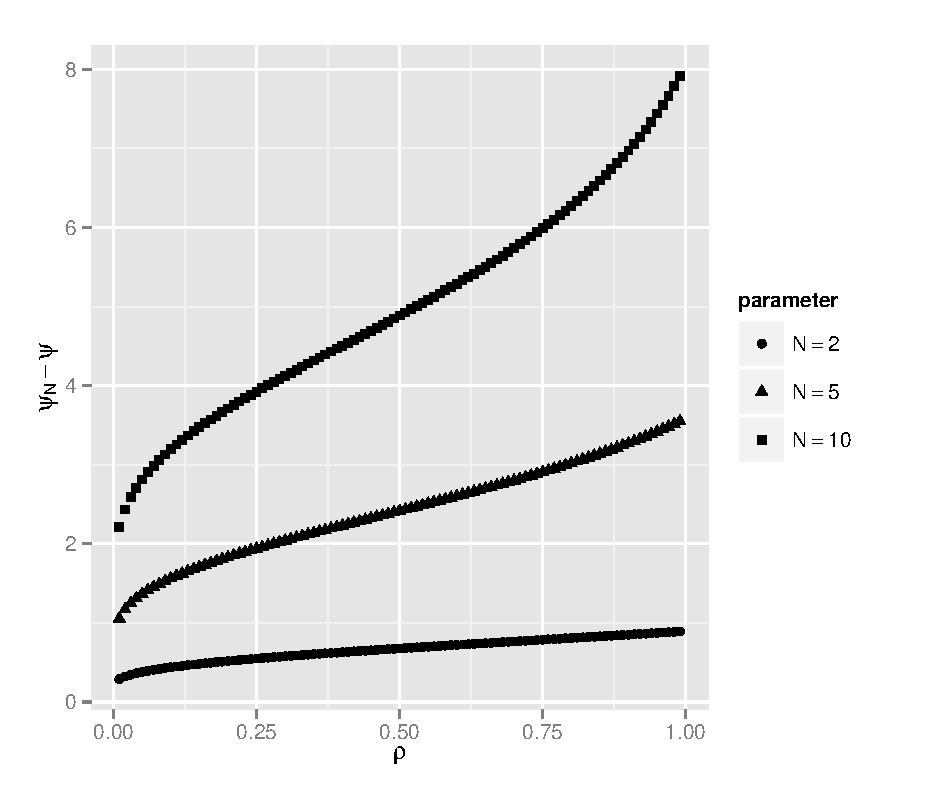
\includegraphics[width=14cm]{backorder_diff.eps}
\caption{改进前后极限成本率之差随$\rho$的变化}
\label{fig:改进前后极限成本率之差}
\end{figure}

图\ref{fig:改进前后极限成本率之差}显示,$\rho$越接近1,改进前后的库存之差越大。我们求出$\rho$接近1时,$\Delta\psi$的极限,可以作为改进效果的上限。设所有需求的到达速率相同,即$p_i=\frac{1}{N}$。
\begin{equation}
\lim_{\rho\to 1}\Delta\psi = h\ln\gamma\lim_{\rho\to 1}\sum_{i=1}^N\left[\frac{1}{\ln\frac{p_i\rho}{1-\rho+p_i\rho}}-\frac{p_i}{\ln\rho}\right]
\label{eq:极限成本率差}
\end{equation}
对公式\ref{eq:极限成本率差}使用洛必达法则,可以得到
\begin{equation}
\lim_{\rho\to 1}\Delta\psi = \frac{1}{2}h(N-1)\ln\frac{h+b}{h}
\label{eq:极限成本率差结果}
\end{equation}
公式\ref{eq:极限成本率差结果}可以作为估算改进效果上限的一种手段。







\section{服务水平约束的影响}

见文献《On the benefits of ...》






